\section[G5: \textit{X-Y} coordinates of a dozen points of \textit{S}]{G5: \textit{X-Y} coordinates of a dozen points of $S$}
This section focuses on the computation and visualization of $X-Y$ coordinates for selected points on the curve SS, leveraging a metric-rectified image from previous stages. The objective is to map curve points from their original image space to a rectified coordinate space, ensuring metric accuracy, and to visualize the adjusted curve points on the rectified image.

\begin{itemize}
    \item \textbf{Rectified Image}: The metric-rectified image (\ref{fig:metricRectificationUsingOneCircle}) obtained in previous steps was loaded as the base for the analysis.
    \item \textbf{Curve SS Points}: Data points defining the curve $S$ were read from input file. These points are assumed to be in the original image's pixel space.
\end{itemize}

A set of known reference points in the original image and their corresponding points in the rectified image were defined. These pairs were used to compute the transformation matrix.

A projective transformation (\texttt{fitgeotrans}) was computed using the reference points from the original and rectified images. This transformation was applied to map the curve $S$ points from the original to the rectified coordinate space. Using the computed transformation, the curve points were rectified.

The rectified image was displayed with the transformed curve $S$ points overlaid in red:

\begin{figure}[H]
    \centering
    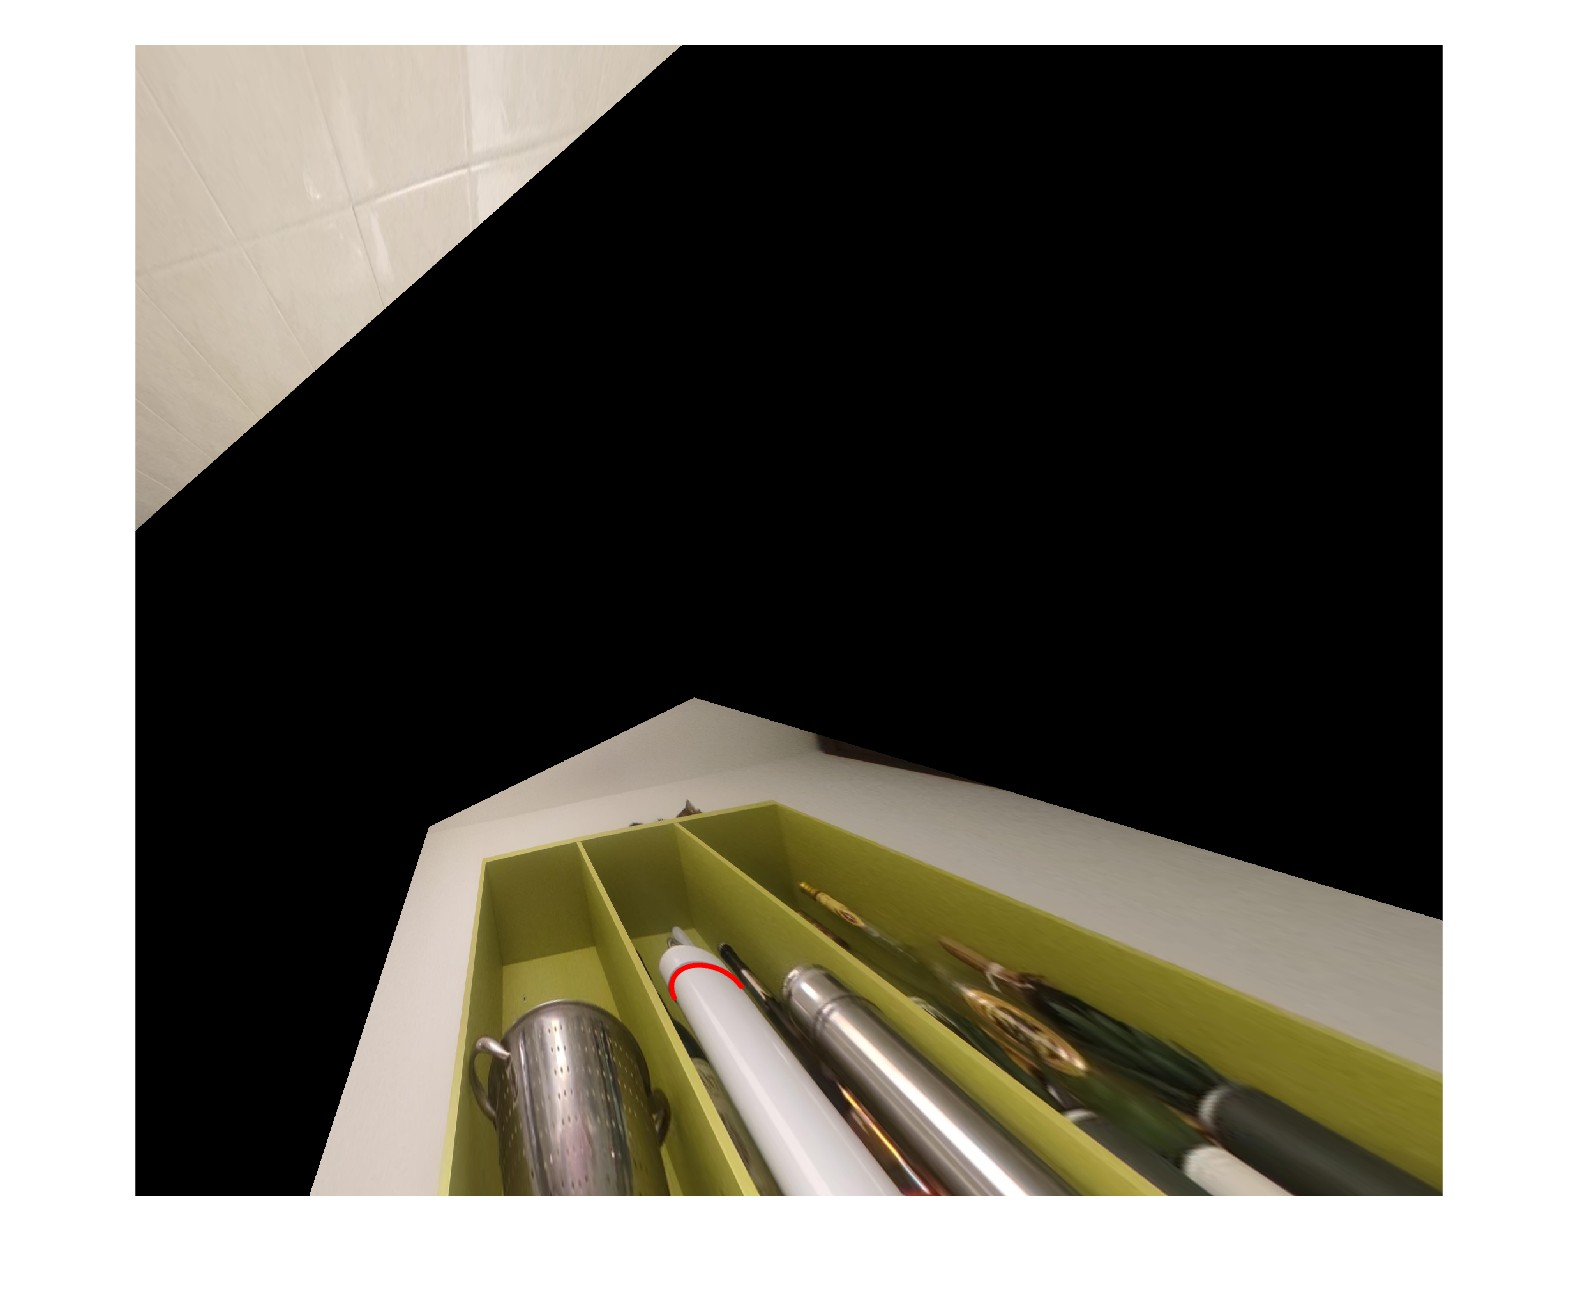
\includegraphics[width=0.7\linewidth]{img/G5/G5_horizontal_metric_rectified_with_S.jpg}
    \caption{Rectified $S$}
    \label{fig:rectifedS}
\end{figure}

To validate the rectification process and transformation accuracy, a selection of random points from the rectified curve $S$ is displayed below:

\begin{table}[h!]
\centering
\begin{tabular}{@{}c c@{}}
\toprule
\textbf{X Coordinate (in pixels)} & \textbf{Y Coordinate (in pixels)} \\ \midrule
5.4979 & 9.5996 \\
5.4950 & 9.6679 \\
6.1065 & 9.5406 \\
5.4942 & 9.6590 \\
5.6008 & 9.4646 \\
6.1350 & 9.5641 \\
5.9547 & 9.4576 \\
5.6890 & 9.4320 \\
5.5107 & 9.7314 \\
5.4937 & 9.6502 \\
6.0864 & 9.5260 \\
5.4936 & 9.6415 \\ \bottomrule
\end{tabular}
\caption{Coordinates of random points from the rectified curve \( S \), scaled by \( 10^3 \).}
\end{table}
